Finite element simulations were carried out using the software
\texttt{COMSOL Multiphysics 4.3 (4.3.0.233)}~\cite{multiphysics1994comsol}.
Though this software's source code is not available for
scrutinous review, our implementation is generic and may be carried out
using other software (e.g. \texttt{OpenFOAM}~\cite{jasak2007openfoam},
\texttt{SU2}~\cite{palacios2013stanford}).  Unless otherwise stated,
implementation specific information is applicable to \comsol.

The simulation is done by solving the steady state incompressible Navier
Stokes equations, neglecting turbulence, using finite element analysis in
two dimensions
\begin{align}
 \rho\left(\mathbf{\dot{u}}\cdot \nabla\right)\mathbf{\dot{u}}
 &=\nabla \cdot \left( -\rho \mathbf{I} + \eta \left(\nabla \mathbf{\dot{u}} +
 \left( \nabla \mathbf{\dot{u}}\right)^\mathrm{T}\right)\right) + \mathbf{F}\\
 \rho \nabla \cdot \mathbf{\dot{u}} &= 0
\end{align}
where $\mathbf{\dot{u}}$ is flow velocity field, $\rho$ is fluid density,
$\eta$ is dynamic viscosity, and $\mathbf{F}$ is the body force per unit
volume.  The computational domain is set up as shown in
\Figure{fig:compgeometry}.  
\begin{figure}[h]
 \centering
 \import{qcm/figures/}{geometry.pdf_tex}
 \caption{Computational geometry for the simulation.}
 \label{fig:compgeometry}
\end{figure}

The left hand side (
\tikz[baseline=-0.75ex]{
 \draw [dash pattern=on 3pt off 2pt on 1pt off 2pt, thick] (0,0) -- (0.5,0);
}) %
is a sliding wall and is given a tangential velocity of $\dot{u}_\perp = \mi
\omega u_0$, where $\omega=2\pi f$ is the angular frequency of oscillation
and $u_0=\SI{1e-2}{\nano\meter}$ is its amplitude.  The top and bottom
(%
\tikz[baseline=-0.75ex]{
 \draw [dash pattern=on 3pt off 1pt, thick] (0,0) -- (0.5,0);
}%
) are given a periodic flow condition such that their pressure difference
is zero.  The right hand side (
\tikz[baseline=-0.75ex]{
 \draw [dash pattern=on 1pt off 1pt, thick] (0,0) -- (0.5,0);
}) %
has a zero-slip condition.  The two materials 1, the particle, and 2, the
medium in domains $D_1$ and $D_2$ are assigned a volume force $\mathbf{F}=\mi \omega \rho
\mathbf{\dot{u}}$,
where $\rho$ is the density of the material, (e.g. $\rho_1 =
\SI{1.06}{\gram\per\centi\meter\cubed}$ for polystyrene and $\rho_2 =
\SI{1}{\gram\per\centi\meter\cubed}$ for water).  Finally. an initial pressure point
constraint of $p_0=0$ is assigned to the point in the bottom right of the
domain.  

The sphere (or, more appropriately, cylinder in 2D) comprising $D_1$ with
diameter $d$ and radius $r$ is located a distance $s>-r$, measured from the
bottom of the sphere, from the oscillating
boundary.  If $s>0$, the sphere does not make contact with the boundary.
If $s\leq0$, the sphere is truncated at the boundary resulting in a finite
contact radius $r_\mathrm{c}$.  It is useful to sample in either domain, so
we either sweep $r_\mathrm{c}$ or $s$, converting between them with
\begin{align}
 r_\mathrm{c}\left(s\right) &= \sqrt{2r-s}\sqrt{s}\\
 s\left(r_\mathrm{c}\right) &= \left(r-\sqrt{r^2-r_\mathrm{c}^2}\right)\sgn\left(r_\mathrm{c}\right)
\end{align}
The number density $N_\mathrm{L}$ was controlled by increasing or
decreasing the height of the domain proportional to the size of the sphere.

The materials in the simulation are assigned a complex dynamic viscosity
$\eta = \eta'-\mi\eta''$.  This is related to the complex bulk modulus
$G=G'+\mi G''$ by
\begin{align}
 \eta = \frac{G}{\mi \omega}
\end{align}
and the loss tangent, the angle between the real and imaginary components
is 
\begin{equation}
 \tan \delta = \frac{G''}{G'}
\end{equation}

Specific to the stationary solver in \comsol, in the
\texttt{Study$\rightarrow$Stationary Solver$\rightarrow$Advanced} window,
``Allow complex-valued output from functions with real input'' was checked.
This, coupled with the complex valued input for the body forces, will
produce shear waves in the simulation.

The mesh settings were calibrated in \comsol~for fluid dynamics with a
maximum mesh size of \SI{1e-9}{\meter} along the oscillating boundary.  All
other meshes were generated automatically.  As for the size of the
computational domain, we find that a height (parallel to the oscillating
boundary) of $h=2d$ and width (perpendicular to the oscillating boundary)  
$w=2d$, minimum of \SI{500}{\nano\meter}, produces consistent results with a
minimum of error and computational resources.

It is important to note that, because the simulation is two dimensional,
what is actually simulated are infinite cylinders rather than spheres.  For
Sauerbrey type viscoelastic films, the influence of this is negligible.
However, for asperity contacts such as spheres, we find that the results,
however qualitatively correct, do not always result in exact numerical
agreement with experiment~\cite{Vittorias2010489}.  An extended simulation
in three dimensions at some point is warranted.

\subsection{Extracting Shifts}
Shifts in frequency, $\df$, and bandwidth (half-width at half maximum),
$\dg$, are computed by evaluating the stress-speed ratio of the oscillating
boundary according to the relationship
\begin{equation}
 \frac{\df+\mi\Delta\Gamma}{f_{\mathrm{F}}}=\frac{\mi}{\pi Z_{\mathrm{q}}}Z_\mathrm{L} =\frac{\mi}{\pi Z_{\mathrm{q}}}\left<\frac{\sigma}{\dot{u}}\right>
\label{eqn:comsolextract}
\end{equation}
where $\sigma$ is the (complex) stress, $\dot{u}$ is the (complex)
velocity, $Z_\mathrm{L}$ is the load impedance, and $\left<\enspace\right>$
denotes a line average along the boundary.  In \comsol, and in the
coordinates of \Figure{fig:compgeometry}, $\sigma$ is 
\texttt{Total stress, y component} (\texttt{v}) and $\dot{u}$ is 
\texttt{Velocity field, y component}, (\texttt{spf.T\_stressy}).  Note that
the stress speed ratio $\left<\sigma/\dot{u}\right>$ is dimensionally equivalent to
specific acoustic impedance, also called ``shock impedance'', sound
pressure over velocity.  In other words, the stress-speed ratio is the
impedance of the film. 

\subsection{Verification Examples}
Here we check the validity of the numerical simulation with examples for
which the QCM's response is well known.

\subsubsection{Evanescent Shear Wave}
Setting up the model as described produces a shear wave which closely
matches theory, as shown in \Figure{fig:suppshearwave}.  An analytic expression
of the evanescent shear wave in a liquid has been reported~\cite{steinem2007piezoelectric} to be 
\begin{equation}
 \frac{u(z)}{u_0} = \exp\left(-\sqrt{\frac{\mi \rho \omega}{\eta}} z\right)
\end{equation}
where $\eta=\eta'-\mi\eta''$ is the complex viscosity, $\rho$ is the density
of the liquid, $\omega$ is the angular frequency of the QCM oscillation,
and $z$ is the spatial extension.  The $1/\me$ penetration depth $\delta$ is
\begin{equation}
 \delta =
 -\left(\Im\left(\sqrt{\frac{\rho\omega}{\mi\eta}}\right)\right)^{-1}
 \label{eqn:suppshearwavedelta}
\end{equation}

With $\rho=\SI{1}{\gram\per\centi\meter\cubed}$ and 
$|\eta|^2=\SI{1}{\milli\pascal\second}$, \Equation{eqn:suppshearwavedelta}
predicts
$\delta\approx\SI{252}{\nano\meter}$.  This is in good agreement with the
simulation data, shown in \Figure{fig:suppshearwave}.

\begin{figure}[h]
 \centering
\pgfplotsset{
 minor tick num=3,
 footnotesize,
 every
 axis/.style={
  xmin=0,xmax=1e-6,ymin=-0.1,ymax=1.1,
  width=0.71\textwidth,height=0.45\textwidth,
  xticklabel style={/pgf/number format/fixed,
                     /pgf/number format/precision=1},
 },
 xlabel = $z$ distance,
 ylabel = $\|\mathbf{\dot{u}}\|$,
 x unit = \si{\micro\meter},
 y unit = a.u.,
 max space between ticks=1000pt,
}
\begin{tikzpicture}[baseline]
\begin{axis}
 \addplot [color=Set14qual1, mark=o, each nth point={5}, only marks ] file {qcm/figures/data/evanescentwave_water_comsol.dat};
 \addlegendentry{simulation}
 \addplot [color=Set14qual2,] file {qcm/figures/data/evanescentwave_water_theory.dat};
 \addlegendentry{theory}
\end{axis}
\end{tikzpicture}
\caption{QCM shear wave decay at \SI{5}{\mega\hertz}, comparison between
simulation and theory.}
\label{fig:suppshearwave}
\end{figure}

\subsubsection{Semi-Infinite Viscoelastic Medium}
A semi-infinite medium will produce a complex response described
by~\cite{kanazawa1985frequency}~\cite{martin1991characterization}
\begin{align}
 \frac{\df+\mi\dg}{f_\mathrm{F}}&=\frac{\mi}{\pi Z_\mathrm{q}}\sqrt{\rho G}\\
                                &= \frac{1}{\pi Z_\mathrm{q}}\frac{\left(-1+\mi\right)}{\sqrt{2}}\sqrt{\omega \rho \eta}
\label{eqn:impeq}
\end{align}

%\Equation{eqn:comsolextract} is equivalent to
$f=\omega/(2\pi)$ is the frequency of the crystal, $\rho$ and $\eta$ are the density and viscosity
of the medium in contact with the crystal, and $\rho_\mathrm{q}$ and
$\mu_\mathrm{q}$ are the density and shear modulus of quartz.  This model
applies for crystals with one side in contact with the viscoelastic
material.  This is related to the dynamic viscosity and shear
modulus by
\begin{align}
\frac{\df+\mi\Delta\Gamma}{f_{\mathrm{F}}}&=\frac{\mi}{\pi Z_{\mathrm{q}}}
\frac{\left(-1+\mi\right)}{\sqrt{2}}\sqrt{\rho\omega\left(\eta'-\mi\eta''\right)}\\
&=\frac{\mi}{\pi Z_{\mathrm{q}}}\sqrt{\rho\left(G'+\mi G''\right)}
\label{eqn:viscoshear}
\end{align}
The simulation geometry was set as described in \Figure{fig:compgeometry}
but without $D_1$ (no sphere).  Extracted values of $\df$ and $\dg$ are
presented in \Figure{fig:viscosweep} as a function of the viscosity $\eta$
of medium 1.  In \Figure{fig:viscosweep}(a) we sweep $\eta'$ for a
Newtonian fluid, $\eta''=0$.  In \Figure{fig:viscosweep}(b) we model a
non-Newtonian sample; $\eta'=\SI{1}{\milli\pascal\second}$ and $\eta''$ is
swept.  The excellent agreement with theory demonstrates that our
simulation is applicable for a wide range of materials.

\begin{figure}[h]
\centering
 \pgfplotsset{
  minor tick num=3,
  footnotesize,
  legend style={font=\footnotesize},
  every axis/.style={
   height=0.50\textwidth,
   width=0.50\textwidth,
   thick,
   %ymin = -0.0003,
   %ymax =  0.0003,
   %xmin = -0.0001,
   %xmax = 0.0038,
  },
  max space between ticks=50pt,
 }
 \begin{tabular}{cc}
 \begin{tikzpicture}[baseline]
  \pgfplotstableread{qcm/figures/data/gksimulation.dat}{\datatablea}
  \pgfplotstableread{qcm/figures/data/gktheory.dat}{\datatableb}
  \begin{axis}[ 
    xlabel = real viscosity $\eta'$,
    x unit = \si{\pascal\second},
    scaled y ticks=base 10:-3,
    ylabel = {$\df$, $\dg$},
    y unit = \si{hertz},
    ylabel absolute,
    restrict x to domain={-0.01:0.6e-2},
    ylabel style={
      %at={(yticklabel* cs:0.25)},
      %xshift=36pt,
      anchor=center,
     },
   ]
   %\addplot table [ y expr=\thisrowno{1} ] {\datatablea};
   \addplot [color=Set14qual1, mark=,] table [ y expr=\thisrowno{1} ] {\datatableb};
   \addplot [color=Set14qual1, mark=, densely dashed] table [ y expr=\thisrowno{2} ] {\datatableb};

   \addplot [color=Set14qual1, mark=o, only marks] table [ y expr=\thisrowno{1} ] {\datatablea};
   \addplot [color=Set14qual1, mark=o, only marks] table [ y expr=\thisrowno{2} ] {\datatablea};

   \draw [color=gray,dashed,semithick] (axis cs:-0.0001,0) -- (axis cs:6e-2,0);
   \node[anchor=north west] at (yticklabel* cs:1) {(a)};

  \end{axis}
 \end{tikzpicture}
 &
 \begin{tikzpicture}[baseline]
  \pgfplotstableread{qcm/figures/data/gksimulation2.dat}{\datatablea}
  \pgfplotstableread{qcm/figures/data/gktheory2.dat}{\datatableb}
  \begin{axis}[ 
    xlabel = imaginary viscosity $\eta''$,
    x unit = \si{\pascal\second},
    scaled y ticks=base 10:-3,
    ylabel = ,
    y unit = ,
    ylabel absolute,
    %restrict x to domain={0:0.6e-2},
    legend to name=named,
    legend columns=-1,
%    legend entries={%
%     $\df$ theory,
%     $\dg$ theory,
%     $\df$ simulation,
%     $\dg$ simulation,
%    },
    ylabel style={
      %at={(yticklabel* cs:0.25)},
      %xshift=36pt,
      anchor=center,
     },
   ]
   \addplot [color=Set14qual1, mark=,] table [ y expr=\thisrowno{1} ] {\datatableb};
   \addlegendentry{$\df$ theory~~}
   \addplot [color=Set14qual1, mark=, densely dashed] table [ y expr=\thisrowno{2} ] {\datatableb};
   \addlegendentry{$\dg$ theory~~}

   \addplot [color=Set14qual1, mark=o, only marks] table [ y expr=\thisrowno{1} ] {\datatablea};
   \addlegendentry{$\df$ simulation~~}
   \addplot [color=Set14qual1, mark=o, only marks] table [ y expr=\thisrowno{2} ] {\datatablea};
   \addlegendentry{$\dg$ simulation~~}

   \draw [color=gray,dashed,semithick] (axis cs:-0.001,0) -- (axis cs:6e-2,0);
   \node[anchor=north west] at (yticklabel* cs:1) {(b)};

  \end{axis}
 \end{tikzpicture}
 \\[1.5cm]
 %\multicolumn{2}{c}{ \ref{named} }
\end{tabular}
\caption{Comparison of $\df$ and $\dg$ verses viscosity $\eta$ for both the
 finite element simulation and \Equation{eqn:impeq}.  (a) $\eta''=0$ and
 $\eta'$ is swept (a Newtonian liquid).  (b)
$\eta'=\SI{1}{\milli\pascal\second}$ and $\eta''$ is swept.}
\label{fig:viscosweep}
\end{figure}

It is of note that our Navier-Stokes approach (which solves for
$\dot{\mathbf{u}}$) does not converge in the limit of a perfectly elastic
material, e.g. $G=G'$ or $\eta=\eta''$; these systems are typically
solved for $\mathbf{u}$.  It is perhaps possible to couple these two
domains, but we have not attempted to do so.


\subsection{Theory and Modeling}
\label{sec:theoryandmodeling}
\subsection{Finite Element Modeling}
%\label{sec:simulation}
To elucidate QCM behavior for samples with discrete particles, we have
performed 2D finite element simulations based on steady state solutions to
the incompressible Navier-Stokes equations.  This model and its
implementation are described in Supplementary Note 2.  The
simulation is setup as depicted in \mbox{\Figure{fig:lowersphere}(a-c)}.  Particles
are represented as spheres (or rather cylinders, in 2D, see Supplementary
Figure 1) which are moved
towards a tangentially oscillating boundary at the bottom of the
computational domain, representing the QCM surface.  Periodic conditions
are imposed on the left and right boundaries such that the ratio of the
domain width to the particle size determines the surface coverage and thus
$N_\mathrm{L}$.  As the particle intersects the oscillating boundary it is
truncated; we identify this truncation with a finite contact radius
$r_\mathrm{c}$ in terms of contact mechanics.
\begin{figure}[ht]
\centering
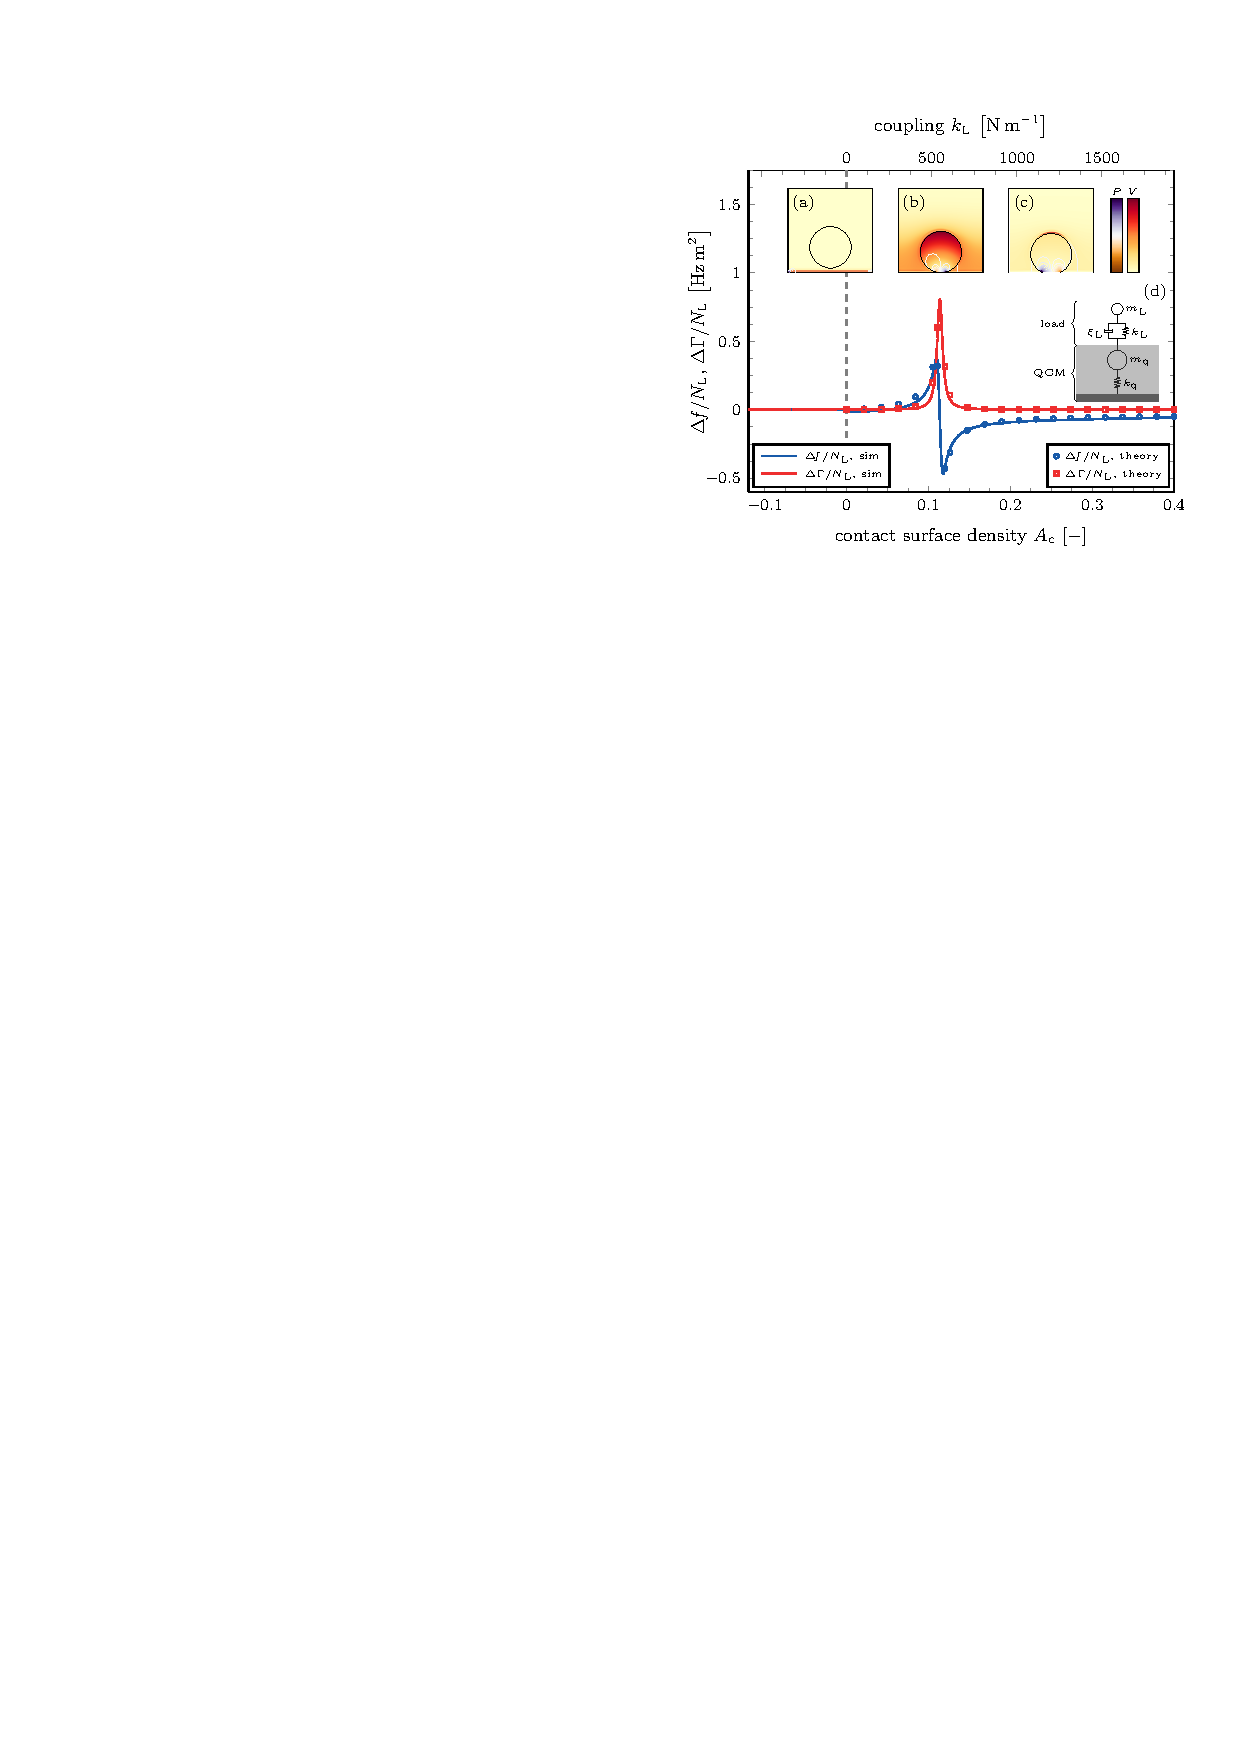
\includegraphics{qcm/figures/figure3.pdf}
\caption{%
Simulation of the CF-QCM behavior.
Finite element simulation for a \SI{10}{\micro\meter} polystyrene
sphere (cylinder in 2D) as a function of contact surface density 
$A_\mathrm{c}$.  Negative values of $A_\mathrm{c}$ indicate positive
separation from the surface.  Discussion in the text. (a-c): Density plot
of the pressure $P$ and velocity $U$ distributions. Units are normalized.
Note that in all situations with finite contact radius, 
stress is annularly distributed around the edge of the contact as per the
Mindlin model~\cite{kumacheva1998interfacial}.
(main plot): Shifts in $\df$ and $\dg$.
(d): Mechanical model based on coupled oscillators. Points on the plot are
a best fit of the mechanical model to the simulation.}
\label{fig:lowersphere}
\end{figure}

A plot of the simulated response in frequency and bandwidth for a
\SI{10}{\micro\meter} particle is depicted in \Figure{fig:lowersphere}.
The spheres were modeled as polystyrene with density
$\rho=\SI{1.06}{\gram\per\centi\meter\cubed}$, shear modulus
$|G_\mathrm{L}|=\SI{1.3}{\giga\pascal}$, and loss tangent $\tan \delta =
0.001$.  The spheres are in water with density
\SI{1.0}{\gram\per\centi\meter\cubed} and viscosity
\SI{1.0}{\milli\pascal\second}.  The shifts in $\df$ and $\dg$ are plotted
as a function of a dimensionless contact surface density $A_\mathrm{c}$,
defined as the contact area of the sample per unit area on the oscillating
boundary. 

The behavior of the simulation closely matches
experimental observations.  As the sphere approaches and makes (weak)
contact with the oscillating boundary, a \textit{positive} shift in both
frequency and bandwidth is observed.  As the contact radius increases, the
sphere becomes more strongly coupled to the boundary. The amount of energy
dissipated into the particle increases until $\dg$ reaches a maximum and
$\df$ experiences a zero crossing.  The limiting case sees a rigid
attachment and the common \textit{negative} frequency shift proportional to
mass adsorption takes hold.  
% say here and in the supplement that the velocity component has some phase
% thing

There are two aspects of the simulation that deserve additional
consideration:
\begin{inparaenum}[(1)]
\item positive shifts in $\df$ and $\dg$ begin 
before physical contact with the oscillating boundary and 
\item for smaller particles $\dg>\df$ while for
larger particles $\df>\dg$.
\end{inparaenum}
The experiment shows the same behavior, as evidenced in
\Table{tbl:particlesize}.  We note however that the procedure of truncation
and its interpretation as finite contact radius in the framework of contact
mechanics utilized here on discrete objects are more accurate for larger
particles (\SI{10}{\micro\meter}, as shown in \Figure{fig:lowersphere})
than smaller ones.  We explain this in the following way.
It is known in
the context of DVLO theory~\cite{israelachvili2011intermolecular} that a
micron-sized polystyrene sphere in water near a similarly charged gold
surface will experience a repulsive force due to electrostatic double-layer
effects~\cite{alexander1987hydrodynamic}~\cite{flicker1993quantifying}.
The balance between this and the gravitational force determines the height
at which the particle will be at equilibrium above the surface.  For the
relevant material
parameters~\cite{israelachvili2011intermolecular}~\cite{sharma1992factors}
we find that, even at \SI{90}{g}, the smaller \num{1} and
\SI{2}{\micro\meter} particles never make contact with the surface, but
``hover'' at separations of approximately
\SIrange{0.3}{0.15}{\micro\meter}.  At nonzero separations we posit that
the sphere-surface coupling, being mediated by a viscous liquid, will be
dominated by loss, hence $\dg>\df$.  On the other hand, larger particles
($\sim\SI{10}{\micro\meter}$ and above) with significant mass will overcome
the double-layer forces and make contact with the QCM through a finite
contact radius.  In this case the coupling losses decrease and $\df>\dg$.

\subsection{Mechanical Model}
\label{sec:mechanicalmodel}
Without mention of the actual physics of the coupling, we observe that the
finite element simulation, as well as the experimental data, follow a simple
mechanical model based on coupled
oscillators~\cite{dybwad1985sensitive}~\cite{olsson2012probing}.  The
arrangement of this mass-spring-dashpot mechanical model is shown in
\Figure{fig:lowersphere}(d).  Here, the resonance of the quartz crystal
$\omegaq^2=\kq/\mq$ is coupled to a sample load with mass $\ml$ though a
parallel spring $\kl$ and dashpot $\xil$ (Voigt
model~\cite{sips1950mechanical}).  Note that $\kl$ is not an actual spring; it
is simply a coupling strength between two oscillators.  The same is true for
$\xil$.  $\ml$ is an actual mass, though in this model it represents a
Sauerbrey mass uncorrected for viscoelastic properties.  

Using the small load approximation, the response of the system as a
function of its coupling $\kl$ can be expressed
as~\cite{steinem2007piezoelectric}
\begin{equation}
\frac{\df + \mi \dg}{f_\mathrm{F}} = \frac{N_\mathrm{L}}{\pi
\mathrm{Z}_\mathrm{q}}
\frac{\ml \omegaq \left( \kl + \mi
\omegaq \xil\right) }
{\ml \omegaq^2 - \left(\kl + \mi
\omegaq \xil\right)}
\label{eqn:mastereq}
\end{equation}
where $\mathrm{Z}_\mathrm{q}$ is the acoustic impedance of AT cut quartz,
$f_\mathrm{F}$ is the fundamental frequency of the resonator, and
$N_\mathrm{L}$ is a surface density (number per unit area) for discrete
loads.  \Equation{eqn:mastereq} as a function of $\kl$ reproduces the
response of the finite element simulation in \Figure{fig:lowersphere},
which is a function of contact surface density $A_\mathrm{c}$ (or in
un-normalized terms the contact radius $r_\mathrm{c}$).  A best-fit comparison to 
the finite element simulation is shown as points in conjunction with the simulation
in \Figure{fig:lowersphere}.  See Supplementary Note 3.

The mechanical model has two important limits as a function of the contact
stiffness, $\kl$, known as \textit{strong} and \textit{weak}
coupling.  These limits occur to the left and right of a zero crossing in $\df$ at
$k_\mathrm{zc}=\omegaq^2 \ml$.

\vspace{-\baselineskip}
\vspace{-\parskip}
\begin{align}
\frac{\df}{f_\mathrm{F}}&= 
\frac{N_\mathrm{L} \kl}
{\omegaq\pi \mathrm{Z}_\mathrm{q}}
&\,&\left(\text{weak,}\quad \kl\ll \ml
\omegaq^2\right)
\label{eqn:couplinguy1}
\\
\frac{\df}{f_\mathrm{F}}&=  -\frac{N_\mathrm{L}
\ml \omegaq}{\pi Z_\mathrm{q}}
&\,&\left(\text{strong,}\quad \kl\gg \ml
\omegaq^2\right)
\label{eqn:couplinguy2}
\end{align}
where we have made the approximation that
$\xil\ll\kl$.~\cite{steinem2007piezoelectric}


Strong coupling is identified with mass loading
(Sauerbrey~\cite{sauerbrey1959verwendung} behavior) and a \textit{negative}
frequency shift linearly proportional $\ml$.  This behavior is the
one which is most commonly associated with QCM measurements.  Physically
this situation is identified with a coupling rigid enough such that
the particle takes part in the oscillation of the QCM.
In the
opposite limit is weak coupling, also called inertial
loading~\cite{dybwad1985sensitive}, and is identified by a \textit{positive}
frequency shift independent of the mass and linearly proportional
to $\kl$.  Here, the coupling is sufficiently weak such that the particle
remains at rest in the labratory frame.  It is ``clamped'' by its own
inertia.~\cite{du2008role}

%This mechanical model fully describes the behavior of the finite element simulations
%for larger ($d\gtrsim\SI{5}{\micro\meter}$) particles, but fails in the
%limit of smaller particles.

Experiments with nanoindentation probes operating on QCMs in the gas
phase~\cite{borovsky2001measuring}, where micron sized spherical tips are
pressed against the sensor surface, have observed the same positive
frequency shift as a function of applied force,  which is identified with
the lateral (sphere-plate) Hertzian spring constant.  We conjecture that
similar behavior will be observed in the liquid phase: the centrifugal load
will primarily act on $\kl$.  We now turn to discussion of how certain
sample parameters can be extracted using this model.

\section{Discussion}
\label{sec:discussion}
The response of the QCM for different load situations under centrifugal
force exhibits a rich and complex set of behavior. Interpretation of all
signals will require experiments beyond the scope of this
manuscript, but we comment on a few examples where our
preliminary data can be predictive within the general model we have set forth.

\subsection{Sample Viscoelasticity}
\label{sec:sampleviscoelasticity}
Finally, we comment on the potential of the CF-QCM technique to be
sensitive to different viscoelastic properties of discrete samples.  While
the mechanical properties seen in biomaterials spans an enormous
range~\cite{meyers2008biological}, we choose three general categories to
highlight potentially interesting sensor responses.  As per
\Figure{fig:multisweep} these are: cells~\cite{li2008thickness}, agarose
microparticles~\cite{li2011surface}~\cite{patra2009viscoelastic}, and
protein microcrystals~\cite{zamiri2009modeling}.  Each is treated in the
finite element simulation as a discrete sphere, with complex shear modulus
$G_\mathrm{L}=G_\mathrm{L}'+G_\mathrm{L}''$, where $G_\mathrm{L}'$ is the
storage modulus related to elasticity, and $G_\mathrm{L}''$ is the loss
modulus related to viscosity.  $G_\mathrm{L}$ is related to viscosity
$\eta_\mathrm{L}$ by $\eta_\mathrm{L}=G_\mathrm{L}/(\mi\omegaq)$.  The
shifts in frequency $\df$ and bandwidth $\dg$ are again plotted as a function of
the dimensionless contact surface density $A_\mathrm{c}$.
A fictitious negative $A_\mathrm{c}$
is identified with a finite separation distance from the
simulated QCM surface.  In all cases the coverage ratio was
\SI{50}{\percent}, and furthermore we assume that centrifugal force will act to
``push'' the sample into the QCM surface, increasing $A_\mathrm{c}$ and
thus the rigidity of its contact with the QCM.
\begin{figure}[ht]
 \centering
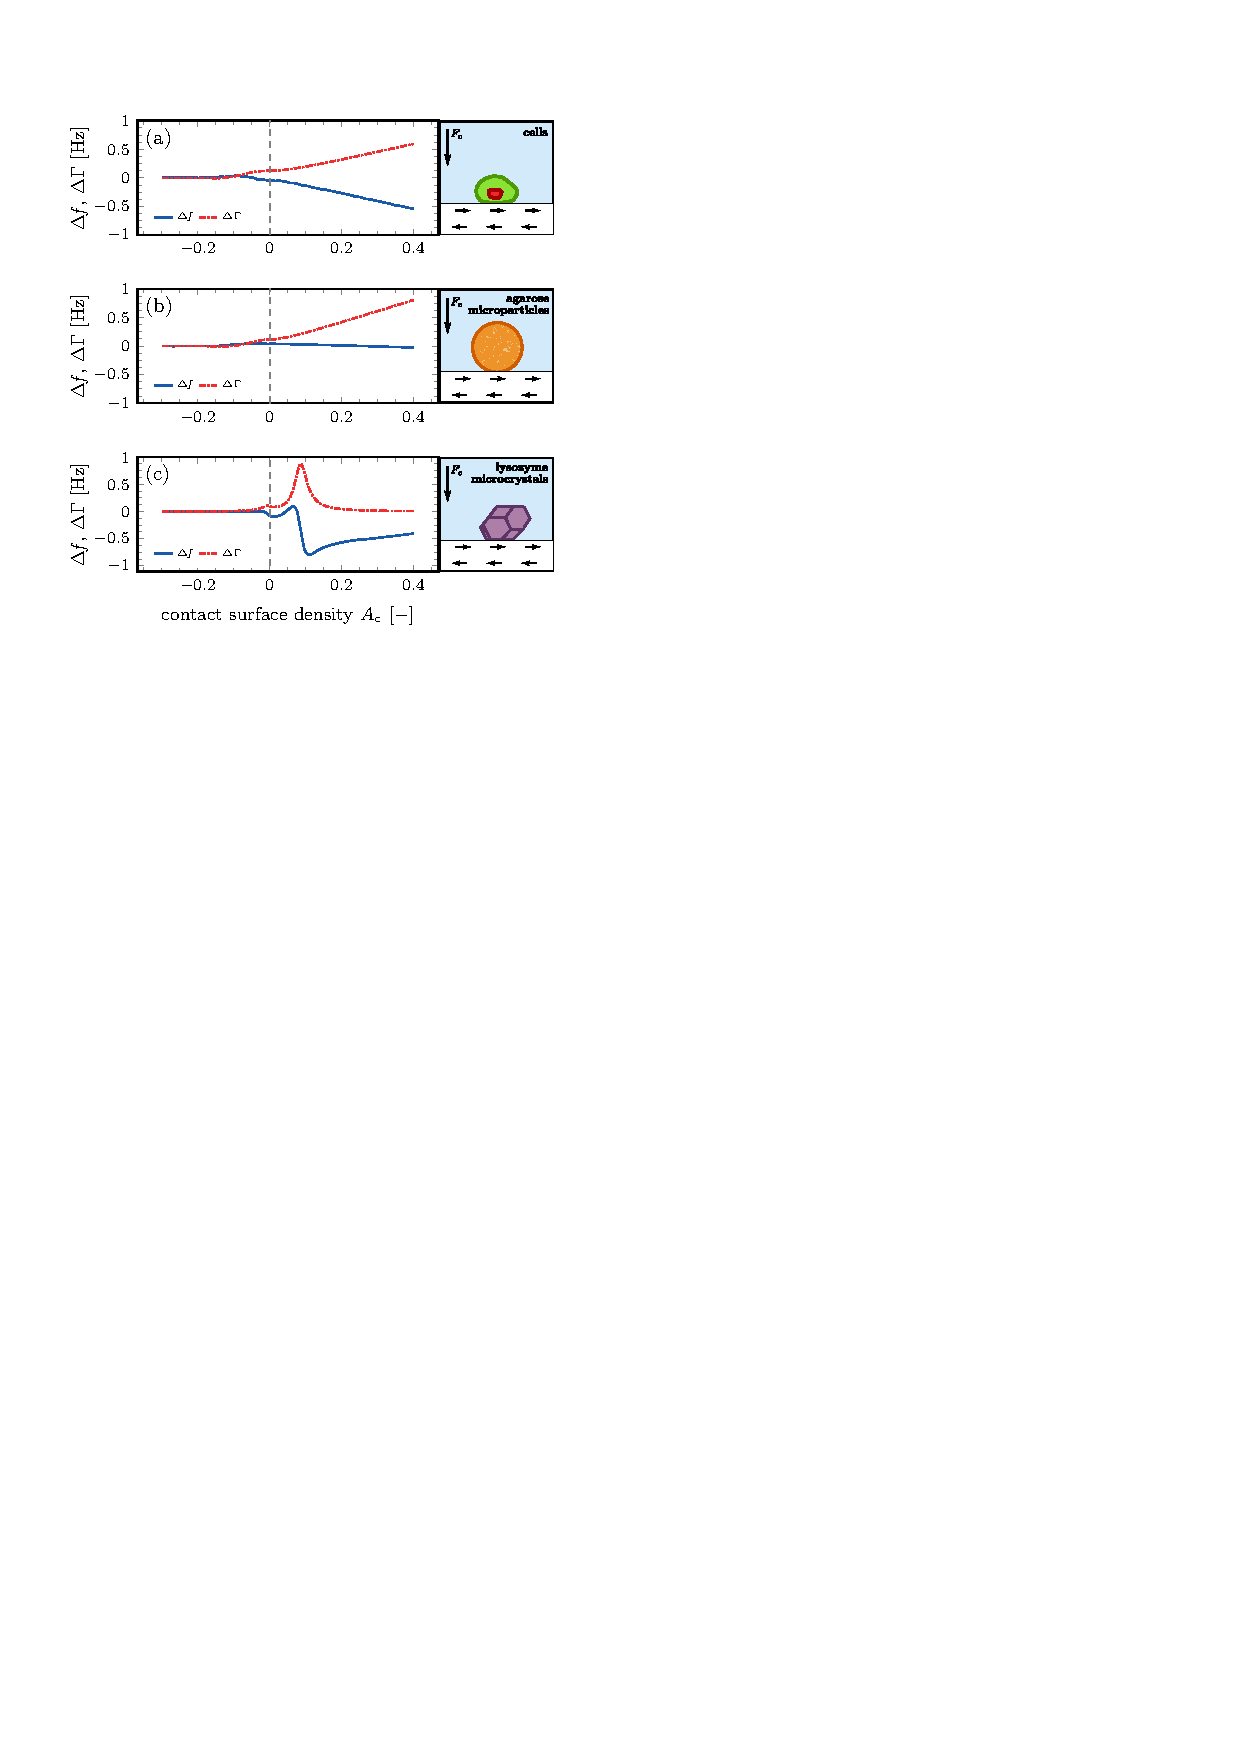
\includegraphics{qcm/figures/figure5.pdf}
\caption{Simulated response for different materials.  Finite element simulation of normalized $\df$ and $\dg$ for three
 categories of samples as a function of contact surface density, 
 $A_\mathrm{c}$.
 Negative values indicate the sample has not made contact with the sensor
 surface.
 The samples are (a) cells, $G_\mathrm{L}=\SI{10+50i}{\kilo\pascal}$, (b)
 agarose microparticles, $G_\mathrm{L}=\SI{78+78i}{\kilo\pascal}$ and (c) lysozyme
 microcrystals, $G_\mathrm{L}=\SI{0.659+0.235i}{\giga\pascal}$.  }
\label{fig:multisweep}
\end{figure}

As can be seen, the simulated response of the CF-QCM is markedly different
in each case. Cells, shown in \Figure{fig:multisweep}(a), are assigned a
shear modulus of $G_\mathrm{L}=\SI{10+50i}{\kilo\pascal}$ and density
$\rho_\mathrm{L}$ equal to the surrounding liquid medium.  The high loss
modulus and low storage modulus predict the cell will exhibit shifts
characteristic of a viscous fluid.  Likewise, the simulation shows $\df$
and $\dg$ decrease and increase linearly proportional to the contact
parameter, beginning before physical contact occurs.  The proportionality
is a simple function of the shear modulus and density in the
semi-infinite approximation~\cite{flanigan2000contact}~\cite{kanazawa1985frequency}
\begin{equation}
 \frac{\df+\mi\dg}{f_\mathrm{F}}=\frac{\mi}{\pi Z_\mathrm{q}}\sqrt{\rho_\mathrm{L} G_\mathrm{L}}
 \left(A_\mathrm{c}\right)
\end{equation}
 Cells in and of
themselves span a large range of viscoelastic properties which have been
demonstrated to be predictive for diseases such as
cancer~\cite{rebelo2013comparison}.  If one knows the way with which
$A_\mathrm{c}$ is modulated by an applied force (e.g. viscoelastic
compliance), linear fitting to
the CF-QCM response will recover $G_\mathrm{L}$ or $\rho_\mathrm{L}$.

Next, \Figure{fig:multisweep}(b) shows the simulated response of agarose
microparticles with a complex shear modulus of
$G_\mathrm{L}=\SI{78+78i}{\kilo\pascal}$. Again the density was assumed to
be the same as the surrounding medium.  Similar to the viscous behavior of
cells, $\dg$ decreases linearly with $A_\mathrm{c}$.  In this
sample however, an equally large elastic term, $G'_\mathrm{L}$, precludes
the equally linear decrease in $\df$ seen for cells.  Instead, $\df$ increases
slightly before contact and decreases slightly.

At the end of the spectrum, \Figure{fig:multisweep}(c) are lysozyme
microcrystals.  These microcrystals are ``hard'', having been assigned a
complex shear modulus of $G_\mathrm{L}=\SI{0.659+0.235i}{\giga\pascal}$.
The response of these is similar to what we experimentally observe with
polystyrene microparticles ($G_\mathrm{L}=\SI{1.3}{\giga\pascal}$).  When
the microcrystal enters the acoustic evanescent wave, there is an initial
negative shift as the effective viscosity-density product increases.  At
small contact parameters there is a positive shift in $\df$ and $\dg$.
Increasing the contact parameter, $\dg$ sees a maximum and $\df$ a zero
crossing.  As the microcrystal becomes strongly coupled to the QCM, the
familiar negative $\df$ is recovered which, as in \Figure{fig:circlefit},
can be used to determine the particle size or mass.

\subsection{Conclusion}
\label{sec:conclusion}
We have observed the QCM sensorgram under the influence of centrifugal force
for samples such as DNA monolayers, free discrete polystyrene particles,
and particles tethered to the QCM electrode with lambda DNA.  We present
simulations and a theoretical framework to interpret the QCM signals in the
context of the sample's properties.

The data presented thus far points to a potentially interesting avenue for
the investigation of force on biomolecules using a quartz crystal
microbalance.  In addition to the data discussed, we have also observed
other types of signals in some of our datasets within the overall trend
shown here, which we suspect may be related to ionic
transport~\cite{tolman1911electromotive}~\cite{des1893unpolarisirbare}, the
conformal state of DNA, and nonlinear viscoelastic behavior.  Objects such
as microparticles attached or tethered to a biopolymer on the QCM surface
become inertial transducers through which one can extract mechanical and
thermodynamic properties of the macromolecules. Furthermore, the technique
is applicable to microscopic biological objects such as viruses, bacteria,
and cells where measurements of mechanical properties and their changes
have been directly linked to
disease~\cite{merkel1989molecular}~\cite{yeri2009mutation}~\cite{tevet2011friction}.

The enhanced signal for most samples under centrifugal load points to a
interesting avenue of increasing the sensitivity of a state of the art QCM
biosensor.  This is true even with the present state of our instrument,
which is limited to low-g regimes when compared to other commercial
centrifuges. With operation below \SI{90}{g}, we have observed sensitivity
increases corresponding to changes of \SI{10}{\percent} in the
density-viscosity product for viscoelastic loads, and up to a factor of 10
increase in sensitivity for discrete particles.  However, there is no
technical reason why future incarnations could not spin much faster and
considerably clarify the CF-QCM sensogram.  There are also possibilities in
using this platform in other related modalities such as the
nanotribological effects of sliding friction~\cite{krim1991nanotribology}
caused by orienting the crystal at an angle to the applied centrifugal
force, propelling biomolecules across the surface.

